\documentclass[10.5pt,a4paper,UTF8]{article}
\usepackage{geometry}
\geometry{margin=1in}
\usepackage{booktabs}
\usepackage{minted}
\usepackage{xcolor}
\usepackage{graphicx}
\usepackage{enumitem}
\usepackage{hyperref}
\usepackage{fontspec}
\usepackage{ctex}

\setmonofont{JetBrainsMono-Regular.ttf}[ItalicFont=JetBrainsMono-Italic.ttf,Path=C:/Users/31515/AppData/Local/Microsoft/Windows/Fonts/]
\setminted{breaklines=true, breakanywhere=true, style=colorful, fontsize=\fontsize{9pt}{11}, linenos=true}

\title{计算机网络实验2\\编写数据包捕获程序并对捕获的数据包进行分析}
\author{鲁昕宁 2414015}
\date{\today}

\begin{document}
\begin{titlepage}
\maketitle
\end{titlepage}

\section{实验目的}
用 C++ 和 Npcap 在本机捕获以太网帧，并把解析结果直接显示在窗口里。实验要完成四件事：
\begin{enumerate}[leftmargin=2em]
    \item 了解 Npcap 从用户态接口到内核驱动的结构；
    \item 用 Npcap 枚举网卡、打开设备并读取数据包；
    \item 从每一帧中取出源 MAC 地址、目的 MAC 地址、类型字段，以及类型字段之后的第一个字节；
    \item 不把数据包存到硬盘，只在屏幕上按列显示这些字段。
\end{enumerate}

\section{实验环境}
程序使用 C++17 和 WinUI 3。捕获接口来自 Npcap SDK 1.17 的 \texttt{pcap.h}，运行时链接本机的 Npcap 1.90。用户态库 \texttt{wpcap.dll} 基于 libpcap 1.10.7，驱动文件是 \texttt{npcap.sys}。安装时打开了 WinPcap API 兼容模式，因此程序按 libpcap 的方式调用即可。注册表中的 \texttt{AdminOnly} 为 0，当前用户可以直接打开网卡。

编译环境为 Visual Studio 2022 Professional，平台工具集 v143，Windows SDK \texttt{10.0.22621.0}，Windows App SDK 1.6。工程带自包含运行库。可执行文件是 \texttt{capture.exe}，位于 \texttt{bin/capture}。

\section{Npcap 架构}
Npcap 把抓包分成四层。程序只接触最上面的一层。

\begin{table}[htbp]
\centering
\caption{Npcap 的层次}
\label{tab:stack}
\small
\setlength{\tabcolsep}{4pt}
\begin{tabular}{lll}
\toprule
层次 & 模块 & 本实验用到的动作 \\
\midrule
用户程序 & \texttt{capture.exe} & 选择网卡、解析以太网头、刷新列表 \\
libpcap 兼容接口 & \texttt{wpcap.dll} & \texttt{pcap\_findalldevs}、\texttt{pcap\_open\_live}、\texttt{pcap\_next\_ex} \\
底层接口 & \texttt{Packet.dll} & 把上面的调用交给内核驱动 \\
内核驱动 & \texttt{npcap.sys} & 作为 NDIS 轻量过滤器挂在网卡上，把帧拷进缓冲 \\
\bottomrule
\end{tabular}
\end{table}

\texttt{pcap\_findalldevs} 返回驱动能看到的适配器。名字类似 \texttt{\textbackslash Device\textbackslash NPF\_\{GUID\}}，描述是网卡在系统里的名称。\texttt{pcap\_open\_live} 按这个名字打开一台适配器，并指定每次最多拷贝的字节数、是否混杂模式，以及读操作的超时。打开之后，驱动把经过该网卡的帧放进内核缓冲，\texttt{pcap\_next\_ex} 从缓冲里取出下一帧。超时返回 0，调用 \texttt{pcap\_breakloop} 返回 $-2$。

本程序在打开后检查 \texttt{pcap\_datalink}。只有 \texttt{DLT\_EN10MB} 才按以太网头解析。回环等设备没有这 14 字节头，会在状态行说明并停止，避免把别的链路头误当成 MAC 地址。

\section{以太网帧与程序结构}
\subsection{帧布局}
四个必显字段在以太网帧头中的位置是固定的。前 12 字节是目的 MAC 和源 MAC，各 6 字节。偏移 12 的两个字节是类型字段，按网络字节序合成一个 16 位整数。偏移 14 就是类型字段后第一个字节。

类型字段与协议的对应关系是：\texttt{0x0800} 表示 IPv4，\texttt{0x0806} 表示 ARP，\texttt{0x86DD} 表示 IPv6，\texttt{0x8100} 表示 VLAN。类型字段为 \texttt{0x8100} 时，这一帧带有 VLAN 标记，类型字段后第一个字节是标记控制信息的高字节，内层类型字段还在其后。程序仍按偏移 12 和偏移 14 读取。捕获长度不足 15 字节时，类型字段和类型字段后第一个字节无法取全。这样的帧不进入列表，状态行显示已经跳过多少帧。

\inputminted[firstline=7,lastline=22,linenos,firstnumber=7]{cpp}{core/ethernet.cpp}

类型为 \texttt{0x0800} 时，类型字段后第一个字节是 IPv4 首部的第一个字节。它的高 4 位是版本号，低 4 位是首部长度，单位为 4 字节。首部不含可选项时，这一字节是 \texttt{0x45}，也就是版本 4、首部长 20 字节。类型为 \texttt{0x0806} 时，类型字段后第一个字节是 ARP 硬件类型的高字节。以太网的硬件类型是 1，所以这个字节通常是 \texttt{0x00}。

\subsection{源码目录}
界面和捕获分开。窗口工程只负责下拉框、按钮和列表，Npcap 调用集中在 \texttt{core}。

\begin{minted}{text}
lab2/
  Capture.sln           解决方案
  build.bat             调用 MSBuild 生成 Release x64
  core/
    ethernet.h/.cpp     按偏移解析 MAC、类型和其后第一个字节
    capture.h/.cpp      设备列表、打开网卡、捕获线程
  app/                  WinUI 窗口
    MainWindow.xaml.cpp 网卡、条数、开始、停止和结果列表
  third_party/npcap/    Npcap SDK 1.17
  bin/capture/          可执行文件和自包含运行库
\end{minted}

设备列表在窗口启动时填充。描述字符串经 \texttt{pcap\_init(PCAP\_CHAR\_ENC\_UTF\_8)} 后按 UTF-8 转成宽字符。

\inputminted[firstline=82,lastline=103,linenos,firstnumber=82]{cpp}{core/capture.cpp}

打开网卡时快照长度为 65535，混杂模式打开，读超时 1000 毫秒。超时让捕获线程能在点击停止后从 \texttt{pcap\_next\_ex} 返回。

\inputminted[firstline=121,lastline=138,linenos,firstnumber=121]{cpp}{core/capture.cpp}

捕获循环在单独的线程里运行。条数为 0 时一直读，直到 \texttt{pcap\_breakloop}。每得到一帧就填好一行，通过回调交给窗口。

\inputminted[firstline=154,lastline=204,linenos,firstnumber=154]{cpp}{core/capture.cpp}

\subsection{界面线程}
捕获线程不接触控件。窗口用 \texttt{post} 把追加一行和改状态行排到 UI 线程，和实验 1 的做法相同。窗口关闭时先把 \texttt{open\_} 置假，再停止捕获线程，避免关闭过程中再改已经销毁的控件。

\inputminted[firstline=151,lastline=164,linenos,firstnumber=151]{cpp}{app/MainWindow.xaml.cpp}

工具栏有网卡下拉框、刷新、条数、开始捕获和停止。下方列表的列是序号、长度、目的 MAC、源 MAC、类型和类型后首字节。列表最多保留最近 1000 行，避免长时间捕获时窗口越来越慢。

\section{运行结果}
在 Intel Wi-Fi 6 AX200 上捕获 12 帧，同时用 \texttt{ping 1.1.1.1} 产生流量。状态行显示“捕获结束，共 12 帧”。达到条数后开始按钮恢复可用，列表不再增长。窗口见图~\ref{fig:capture}。

\begin{figure}[htbp]
    \centering
    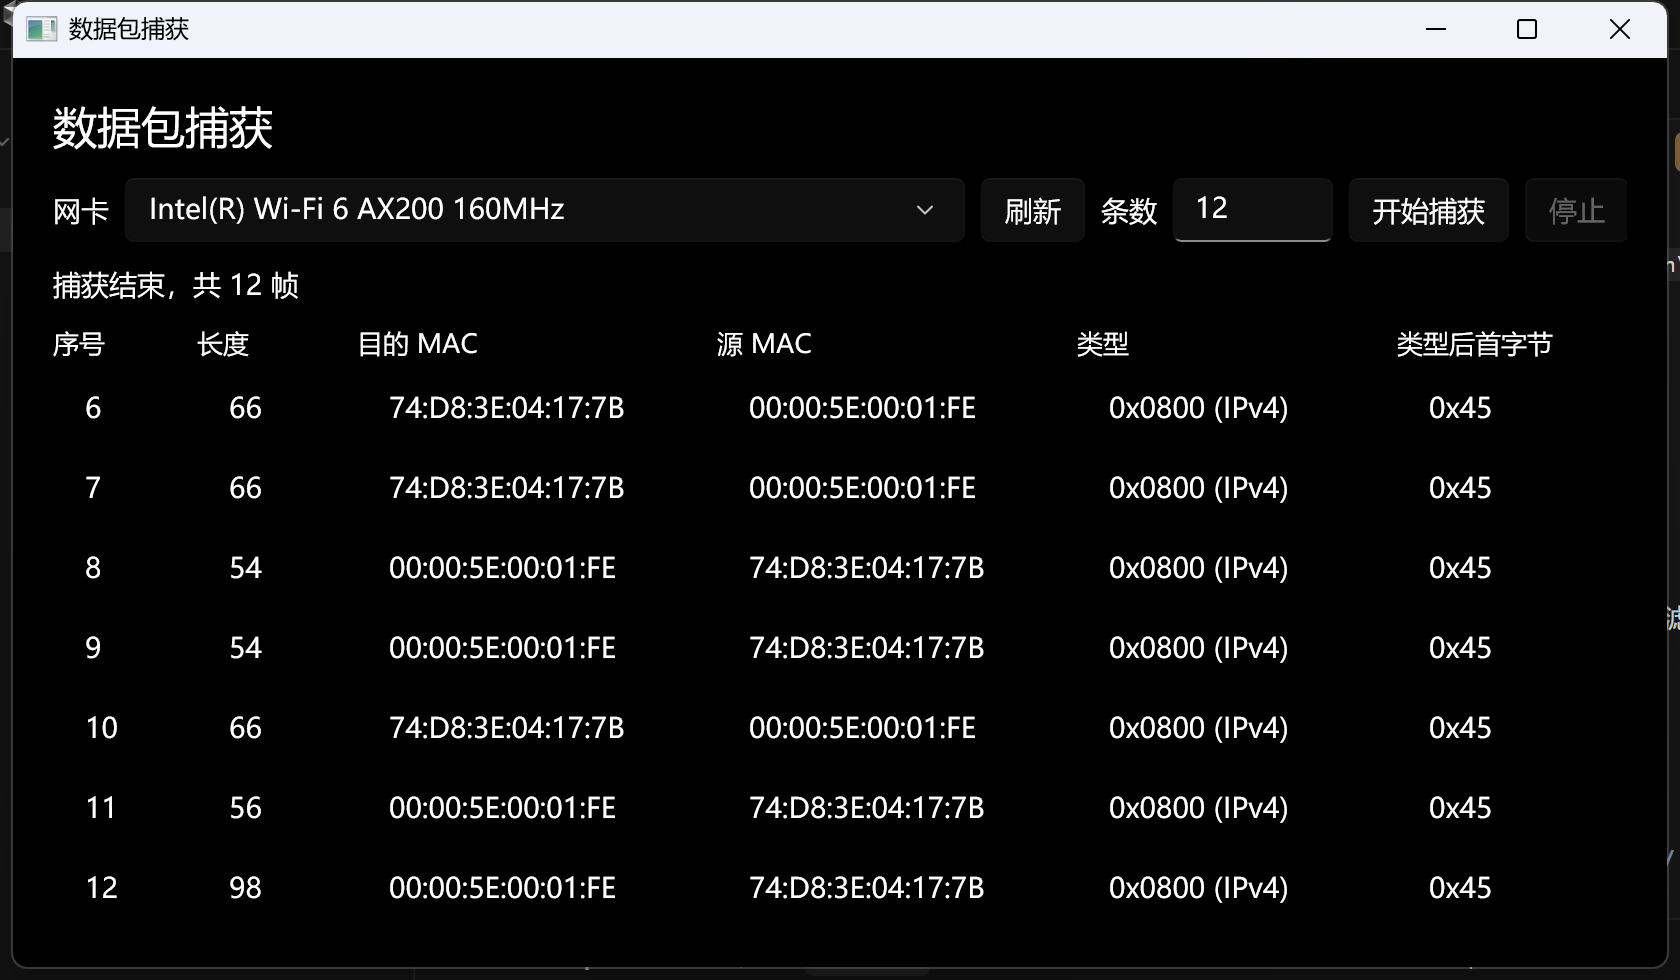
\includegraphics[width=0.92\textwidth]{figure/capture.png}
    \caption{在无线网卡上捕获 12 帧。每行都有目的 MAC、源 MAC、类型和类型后首字节。}
    \label{fig:capture}
\end{figure}

这 12 帧的类型都是 \texttt{0x0800}，类型后的第一个字节都是 \texttt{0x45}。地址只在两台主机之间交替。\texttt{74:D8:3E:04:17:7B} 是本机这块无线网卡的 MAC。\texttt{00:00:5E:00:01:FE} 是 IANA 为 VRRP 保留的虚拟路由器 MAC，这里是无线网关。从本机发出的帧，源地址是网卡 MAC、目的地址是网关；网关发回的帧方向相反。

\begin{table}[htbp]
\centering
\caption{其中四帧}
\label{tab:sample}
\begin{tabular}{llllll}
\toprule
序号 & 长度 & 目的 MAC & 源 MAC & 类型 & 类型后首字节 \\
\midrule
1 & 708 & \texttt{74:D8:3E:04:17:7B} & \texttt{00:00:5E:00:01:FE} & \texttt{0x0800} & \texttt{0x45} \\
2 & 66 & \texttt{00:00:5E:00:01:FE} & \texttt{74:D8:3E:04:17:7B} & \texttt{0x0800} & \texttt{0x45} \\
8 & 54 & \texttt{00:00:5E:00:01:FE} & \texttt{74:D8:3E:04:17:7B} & \texttt{0x0800} & \texttt{0x45} \\
12 & 98 & \texttt{00:00:5E:00:01:FE} & \texttt{74:D8:3E:04:17:7B} & \texttt{0x0800} & \texttt{0x45} \\
\bottomrule
\end{tabular}
\end{table}

\texttt{0x45} 与 IPv4 首部的布局一致：版本号 4，首部长度 5。长度一列从 54 到 708 都有，说明列表显示的是原始帧长，而不是把不同的包裁成一样长。这次捕获没有遇到 ARP。若类型为 \texttt{0x0806}，偏移 14 是硬件类型的高字节，以太网对应的值是 \texttt{0x00}。

\section{结论}
程序通过 Npcap 的 \texttt{wpcap.dll} 枚举网卡、打开以太网设备，并在独立线程里读取帧。窗口按固定偏移显示目的 MAC、源 MAC、类型字段和类型字段之后的第一个字节，不把数据包写到硬盘。在无线网卡上捕获的 12 帧都是发往网关或从网关回来的 IPv4 帧，类型为 \texttt{0x0800}，其后第一个字节为 \texttt{0x45}。
\end{document}
